% called by main.tex
%
\chapter{Resultados II: Ajuste Fino con Predicción Explícita de Nivel}
\label{ch::chapter6}

El capítulo anterior dejó abierta una pregunta que el SFT serializado no puede responder por sí mismo:
¿hasta qué punto la jerarquía mejora cuando el modelo dispone de una señal estructural dedicada en lugar de tener que deducirla del texto generado? En el \texttt{serialized\_sft},
la predicción del nivel es una consecuencia implícita del aprendizaje lingüístico: el modelo aprende que tras ciertos contextos tienden a aparecer ciertos dígitos. No hay nada en la
función de pérdida que le diga explícitamente que ese dígito representa una posición en el árbol jerárquico del YAML. Este capítulo explora una arquitectura alternativa que
supervisa directamente esta variable.

La idea central de este capítulo es sencilla de enunciar: añadir un cabezal adicional que se supervisa directamente sobre la variable \texttt{level}, de modo que el modelo no solo
aprenda a generar texto sino también a predecir la profundidad jerárquica de cada línea como una tarea separada, en línea con la idea general de tratar ciertas salidas como objetos estructurados y no como etiquetas independientes \citep{joachims2009structured, belanger2017spen}. La arquitectura resultante, denominada THM (\textit{Two-Headed Model}),
mantiene la misma superficie de generación que el SFT serializado pero desacopla la señal estructural de la señal textual. El texto y el nivel dejan de competir por el mismo token:
el nivel se convierte en una etiqueta supervisada que el modelo aprende en paralelo a la generación.

Como se verá, la idea es más fácil de enunciar que de hacer funcionar.


%----------------------------------------------------------------------
\section{Motivación: los límites de la supervisión implícita}
\label{sec:ch6_motivation}
%----------------------------------------------------------------------

El \texttt{serialized\_sft} del capítulo anterior logró resultados notables: una tasa de parseo YAML del 98,57\,\% y una coincidencia exacta de nivel del 75,78\,\%. Sin embargo, si
se examina de cerca la naturaleza de esos aciertos, aparece una limitación estructural importante. En el formato \texttt{blocks\_tsv\_v1}, el nivel es simplemente el primer campo de
cada línea generada: un dígito entre 0 y 8, seguido de un tabulador y del contenido textual. El modelo aprende a colocar ese dígito correctamente mediante la misma mecánica con la
que aprende a escribir cualquier otra secuencia de tokens: por asociación contextual y exposición supervisada. Hay señal suficiente en los datos para que el aprendizaje funcione
razonablemente, pero esa señal llega al modelo de forma indirecta, mezclada con la señal de contenido textual.

Este diseño tiene una consecuencia particular ya manifestada en el análisis del capítulo~\ref{ch::chapter3}: el modelo aprende bien los niveles frecuentes (0 a 4)
pero falla de forma sistemática en los niveles profundos (5 a 8). A primera vista, podría atribuirse al desbalanceo de clases: el nivel 5 representa solo el 2,9\,\% de las líneas de
entrenamiento, y el nivel 8 aparece en apenas el 0,1\,\% de ellas. Pero el problema no se reduce a una cuestión de frecuencia. En el SFT serializado, el modelo llega a predecir
dígitos de nivel razonablemente bien en promedio, pero no existe ningún mecanismo que le diga que ese dígito tiene una interpretación estructural: que un nivel 5 implica que la
línea vive bajo cuatro niveles de anidamiento previo, que eso depende de qué recursos se hayan generado antes, y que una predicción incorrecta del nivel no solo produce un dígito
malo sino que puede comprometer toda la estructura del documento.

La hipótesis de partida de este capítulo es que separar la señal de nivel de la señal textual podría ayudar en dos sentidos. Por un lado, la función de pérdida vería el nivel
como una variable explícita a optimizar, no como un subproducto de la generación. Por otro lado, el modelo podría apoyarse en representaciones latentes que, como sugieren los trabajos sobre recuperación de estructura sintáctica en representaciones internas \citep{hewitt2019structural, clark2019bert} y como demostró la sonda
diagnóstica del capítulo~\ref{ch::chapter3}, ya codifican información jerárquica aprovechable. Esa doble intuición es la que motiva el diseño del THM (\textit{Two-Headed Model}).


%----------------------------------------------------------------------
\subsection{Análisis de la señal latente}
\label{sec:ch6_latent_probe}
%----------------------------------------------------------------------

Antes de diseñar una arquitectura con supervisión explícita de nivel, conviene recuperar un resultado del capítulo~\ref{ch::chapter3} que sirvió como comprobación de factibilidad.
El experimento del espacio latente consistió en entrenar clasificadores ligeros sobre las representaciones ocultas del modelo base Qwen2.5-7B-Instruct para predecir la variable
\texttt{level} sin que el modelo hubiera recibido ningún entrenamiento específico para ello. El resultado más sólido, obtenido con un clasificador lineal sobre el estado oculto
en la primera posición token de cada línea (\texttt{line\_first\_token}), alcanzó una exactitud del 78,8\,\% y un error absoluto medio de 0,436 en el split de validación. Ese
resultado no demostraba que el modelo pudiera generar niveles correctos, pero sí que la información estructural ya estaba presente en sus representaciones internas de alguna
forma recuperable.

\begin{figure}[htbp]
\centering
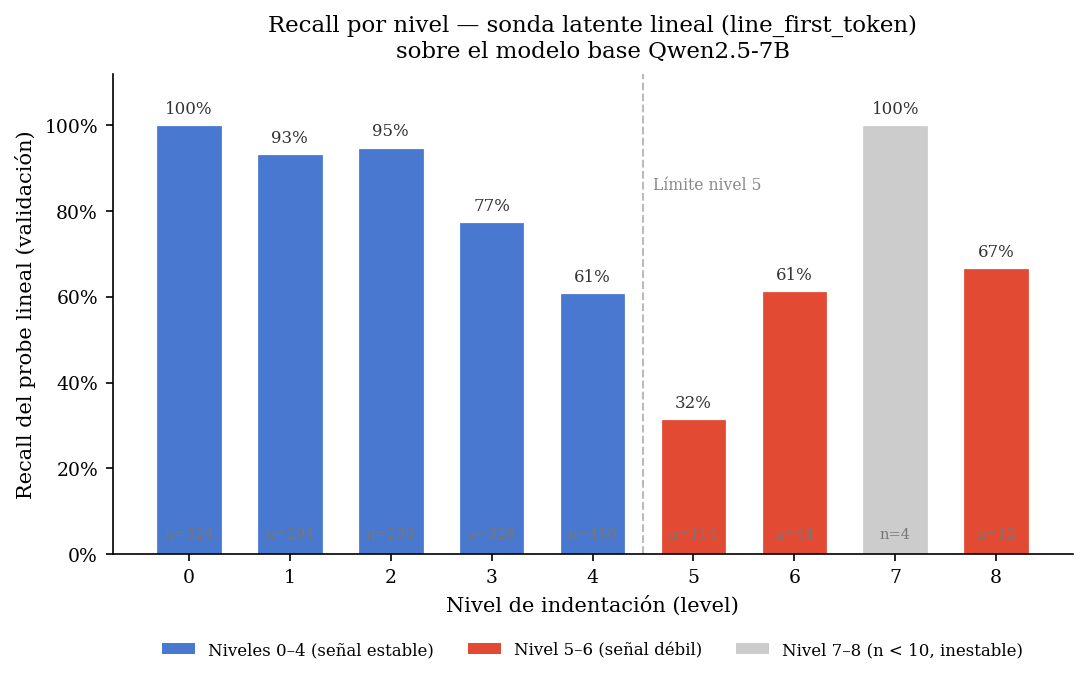
\includegraphics[width=0.78\textwidth]{figures/chapter6/fig6_2_probe_recall_by_level.png}
\caption{Recall por nivel del mejor aproximador lineal (\texttt{line\_first\_token}) sobre las representaciones del modelo base.
         Los niveles 0--4 muestran señal sólida; a partir del nivel 5 el recall cae por debajo del 32\,\%,
         y los niveles 7--8 son inestables por escasez de muestras.}
\label{fig:ch6_probe_recall}
\end{figure}

Sin embargo, como muestra la Figura~\ref{fig:ch6_probe_recall}, la señal no es uniforme a lo largo de la jerarquía. Los niveles 0 a 4 presentan un recall alto y relativamente
estable. A partir del nivel 5 la recuperación cae de forma brusca: la aproximación realizada solo recupera el 31,6\,\% de las instancias de nivel 5 en validación, y los niveles 7 y 8
tienen soporte tan reducido que los resultados son poco fiables. Esto tiene una implicación directa para el diseño: la señal latente existe, pero está concentrada en los niveles
superficiales de la jerarquía. Precisamente los niveles en los que el sistema ya funcionaba razonablemente bien. Para los niveles profundos, que son los más problemáticos, la
sonda confirma que la señal es débil e irregular.

Este patrón orientó varias decisiones de diseño. En particular, la elección de la política de alineación del cabezal de nivel: en lugar de leer el estado oculto en la posición
media de la línea o en el último token, se optó por leer el estado en el momento previo al primer token de cada bloque (\texttt{record\_prefix\_state}). Esta posición capta el
estado del modelo justo antes de comenzar a generar el contenido del bloque, lo que intuitivamente debería concentrar más información estructural sobre el contexto previo que
sobre el contenido en curso.


%----------------------------------------------------------------------
\section{Diseño de la arquitectura de dos cabezales}
\label{sec:ch6_architecture}
%----------------------------------------------------------------------

La idea del THM (\textit{Two-Headed Model}) puede describirse de forma concisa: se toma el modelo base con LoRA y se le añade un segundo cabezal de predicción que opera en paralelo
al cabezal de lenguaje estándar. El cabezal de lenguaje sigue generando el texto de cada bloque token a token, como en cualquier modelo autoregresivo. El cabezal de nivel,
por su parte, toma el estado oculto en una posición específica antes de cada bloque y produce una predicción de clase sobre los nueve niveles posibles (0 a 8). Las dos pérdidas
se combinan de forma aditiva con un coeficiente $\lambda$ que controla el peso relativo de la señal estructural.

\begin{figure}[htbp]
\centering
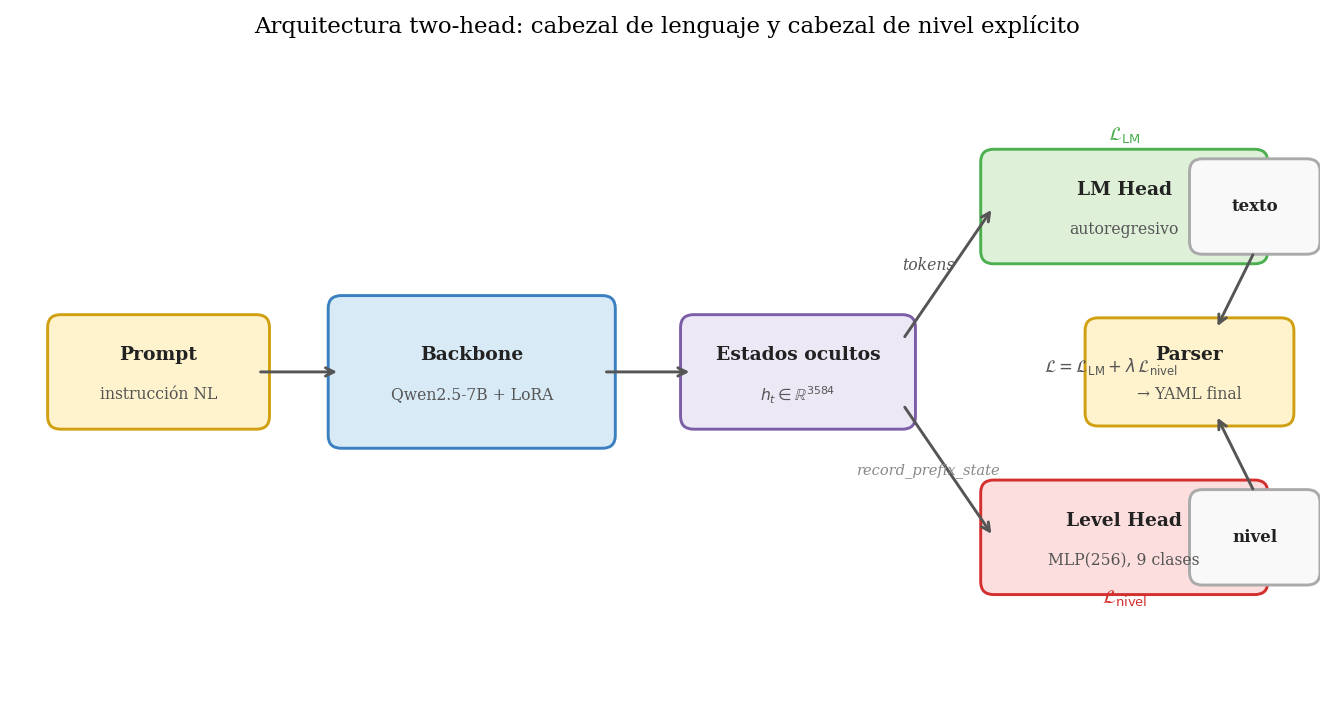
\includegraphics[width=0.88\textwidth]{figures/chapter6/fig6_1_architecture.png}
\caption{Arquitectura del \texttt{THM}: el backbone compartido alimenta simultáneamente el cabezal de lenguaje
         y el cabezal de nivel. La política \texttt{record\_prefix\_state} lee el estado oculto
         justo antes del primer token de cada bloque para supervisar la predicción de nivel.}
\label{fig:ch6_architecture}
\end{figure}

La Figura~\ref{fig:ch6_architecture} ilustra el esquema general. El backbone Qwen2.5-7B con adaptadores LoRA procesa la secuencia de entrada y genera una sucesión de estados
ocultos $h_t \in \mathbb{R}^{3584}$. En cada posición que marca el inicio de un nuevo bloque, el cabezal de nivel lee ese estado oculto y produce una distribución sobre los
nueve niveles de indentación. El cabezal de lenguaje opera de forma estándar sobre todos los estados ocultos de la secuencia, generando el texto del bloque token a token. La
predicción final del nivel proviene exclusivamente del cabezal estructural, no del texto generado: a diferencia del \texttt{serialized\_sft}, el nivel no aparece como un campo en
la superficie de texto del bloque.

\medskip
\noindent La Tabla~\ref{tab:ch6_format_comparison} resume las diferencias de formato entre ambas variantes supervisadas.

\begin{table}[htbp]
\centering
\caption{Comparación de formatos de superficie entre \texttt{serialized\_sft} y \texttt{two\_head\_sft}.
         En la variante de dos cabezales, el campo de nivel desaparece del texto generado y pasa a ser
         una etiqueta supervisada exclusiva del cabezal estructural.}
\label{tab:ch6_format_comparison}
\begin{tabular}{lll}
\toprule
\textbf{Aspecto}            & \textbf{serialized\_sft}                      & \textbf{two\_head\_sft} \\
\midrule
Formato de bloque           & \texttt{blocks\_tsv\_v1}                      & \texttt{content\_blocks\_v1} \\
Nivel en superficie         & Sí (primer campo: \texttt{0}, \texttt{1}\ldots)   & No (etiqueta supervisada) \\
Cabezales de predicción     & 1 (LM head)                                   & 2 (LM head + level head) \\
Política de alineación      & N/A                                           & \texttt{record\_prefix\_state} \\
Pérdida combinada           & $\mathcal{L}_\mathrm{LM}$                    & $\mathcal{L}_\mathrm{LM} + \lambda\,\mathcal{L}_\mathrm{nivel}$ \\
\bottomrule
\end{tabular}
\end{table}

\medskip
El cabezal de nivel es un perceptrón multicapa con una capa oculta de dimensión 256 y dropout del 5\,\%. La función de pérdida es entropía cruzada sobre las nueve clases,
con $\lambda$ = 1 para el peso del cabezal de nivel respecto al cabezal de lenguaje. Los adaptadores LoRA tienen rango 8, escala 16 y se aplican a las proyecciones de atención
(Q, K, V, O). El resto de hiperparámetros de entrenamiento son idénticos a los del \texttt{serialized\_sft}: tasa de aprendizaje $2 \times 10^{-4}$, tres épocas, tamaño de lote
efectivo 8 (acumulación de gradientes sobre batches de tamaño 1), semilla 42 y 426 muestras de entrenamiento. Esta identidad de configuración es deliberada: permite atribuir
cualquier diferencia en resultados a la arquitectura, no a diferencias de entrenamiento.

La transformación del formato de datos es sencilla pero significativa. El formato \texttt{blocks\_tsv\_v1} incluye cuatro columnas por bloque: \texttt{doc\_idx}, \texttt{line\_idx},
\texttt{level} y \texttt{line\_text}. El formato \texttt{content\_blocks\_v1} elimina la columna \texttt{level}: solo contiene \texttt{doc\_idx}, \texttt{line\_idx} y \texttt{line\_text}.
El nivel desaparece por completo de la superficie textual y existe únicamente como etiqueta en el proceso de supervisión. Esto significa que durante la inferencia, el modelo no
puede ``leer'' el nivel que acaba de predecir en el siguiente token: la predicción del cabezal de nivel es invisible para el cabezal de lenguaje.


%----------------------------------------------------------------------
\section{Resultados del experimento base: THM v1}
\label{sec:ch6_twohead_v1}
%----------------------------------------------------------------------

El experimento base (THM v1, checkpoint final, paso 159) se evaluó sobre el split de validación completo de 70 muestras. La Tabla~\ref{tab:ch6_comparison_v1}
presenta la comparativa principal respecto al baseline zero-shot definido en el Capítulo~5. Esta es la comparación relevante en este punto del argumento: antes de confrontar distintas
familias supervisadas entre sí, conviene establecer si el cabezal estructural explícito mejora el punto de partida sin ajuste fino.

\begin{table}[htbp]
\centering
\caption{Comparativa de métricas compartidas en el split de validación: baseline zero-shot vs.\ \texttt{THM v1}
         (70 muestras). La columna $\Delta$ indica \texttt{THM v1} menos baseline; en
         \texttt{average\_level\_mae}, un valor negativo indica mejora porque la métrica es un error.}
\label{tab:ch6_comparison_v1}
\begin{tabular}{lccc}
\toprule
\textbf{Métrica}                          & \textbf{Baseline} & \textbf{THM v1} & $\boldsymbol{\Delta}$ \\
\midrule
Muestras evaluadas                        & 65\,/\,70 & 70\,/\,70 & --- \\
\texttt{yaml\_parse\_success\_rate}       & $30{,}77$\,\%  & $48{,}57$\,\%  & $\mathbf{+17{,}80}$ \\
\texttt{average\_level\_exact\_match\_rate} & $11{,}31$\,\% & $35{,}04$\,\% & $\mathbf{+23{,}73}$ \\
\texttt{average\_level\_mae}              & $0{,}7896$      & $0{,}239$      & $\mathbf{-0{,}551}$ \\
\texttt{average\_line\_text\_f1}          & $20{,}86$\,\%  & $37{,}43$\,\%  & $\mathbf{+16{,}57}$ \\
\texttt{average\_semantic\_key\_f1}       & $27{,}78$\,\%  & $45{,}92$\,\%  & $\mathbf{+18{,}14}$ \\
\texttt{average\_prompt\_requirement\_f1} & $22{,}13$\,\%  & $42{,}06$\,\%  & $\mathbf{+19{,}93}$ \\
\bottomrule
\end{tabular}
\end{table}

\begin{figure}[htbp]
\centering
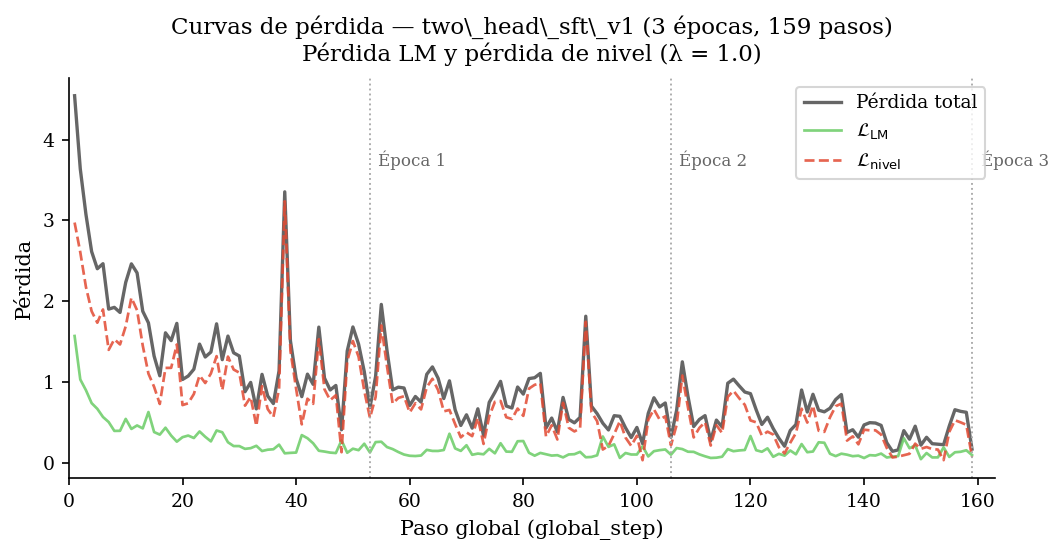
\includegraphics[width=0.88\textwidth]{figures/chapter6/fig6_3_train_loss_twohead.png}
\caption{Curvas de pérdida durante el entrenamiento del \texttt{THM v1}: pérdida total,
         componente LM y componente de nivel ($\lambda$ = 1,0, 3 épocas, 159 pasos globales).}
\label{fig:ch6_train_loss}
\end{figure}

\begin{figure}[htbp]
\centering
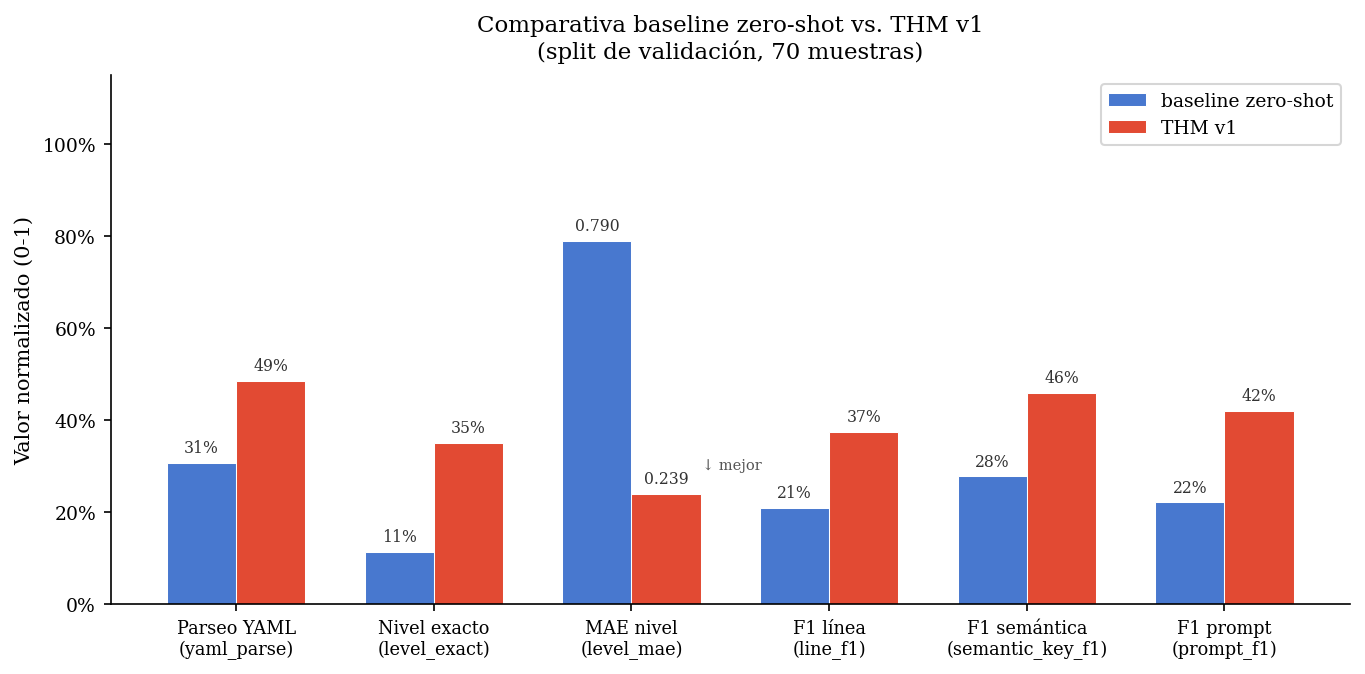
\includegraphics[width=0.88\textwidth]{figures/chapter6/fig6_4_comparison_v1.png}
\caption{Comparativa visual de métricas clave entre el baseline zero-shot y \texttt{THM v1}
         en el split de validación.}
\label{fig:ch6_comparison_bars}
\end{figure}

El resultado es claramente mejor que el punto de partida. El parseo YAML sube de 30,77\,\% a 48,57\,\%, la coincidencia exacta de nivel pasa de 11,31\,\%
a 35,04\,\%, y las métricas de contenido también aumentan: el F1 de línea crece de 20,86\,\% a 37,43\,\%, el F1 semántico de 27,78\,\% a 45,92\,\%, y el F1 de adecuación al prompt
de 22,13\,\% a 42,06\,\%. La señal principal, por tanto, no es que el \texttt{THM v1} sea inferior a otras ramas supervisadas, sino que la separación explícita entre contenido textual
y nivel jerárquico produce una mejora sustantiva frente al modelo sin ajuste.

El error absoluto medio de nivel confirma esa lectura inicial: baja de 0,7896 en el baseline a 0,239 en el \texttt{THM v1}. Ahora bien, debemos de tener en cuenta que el MAE medio 
puede ser bajo si el modelo acierta muchos niveles frecuentes y, al mismo tiempo, ignora por completo la región profunda de la jerarquía.

La Figura~\ref{fig:ch6_train_loss} muestra las curvas de entrenamiento. La pérdida LM desciende de forma estable: caída rápida en la primera época, refinamiento progresivo en las dos
siguientes. La pérdida de nivel, en cambio, presenta un comportamiento diferente: también desciende, pero a un ritmo más lento y sin llegar a los niveles de la pérdida LM. El modelo
aprende simultáneamente ambas tareas, pero no con la misma eficiencia, lo que sugiere que la señal estructural es más difícil de incorporar que la señal textual.


%----------------------------------------------------------------------
\subsection{Colapso hacia los niveles superficiales}
\label{sec:ch6_level_collapse}
%----------------------------------------------------------------------

El diagnóstico más revelador del experimento base no está en las métricas globales sino en la distribución de predicciones de nivel. La Figura~\ref{fig:ch6_level_dist} muestra la
distribución de niveles gold en el split de validación junto con la distribución de los niveles predichos por el cabezal estructural.

\begin{figure}[htbp]
\centering
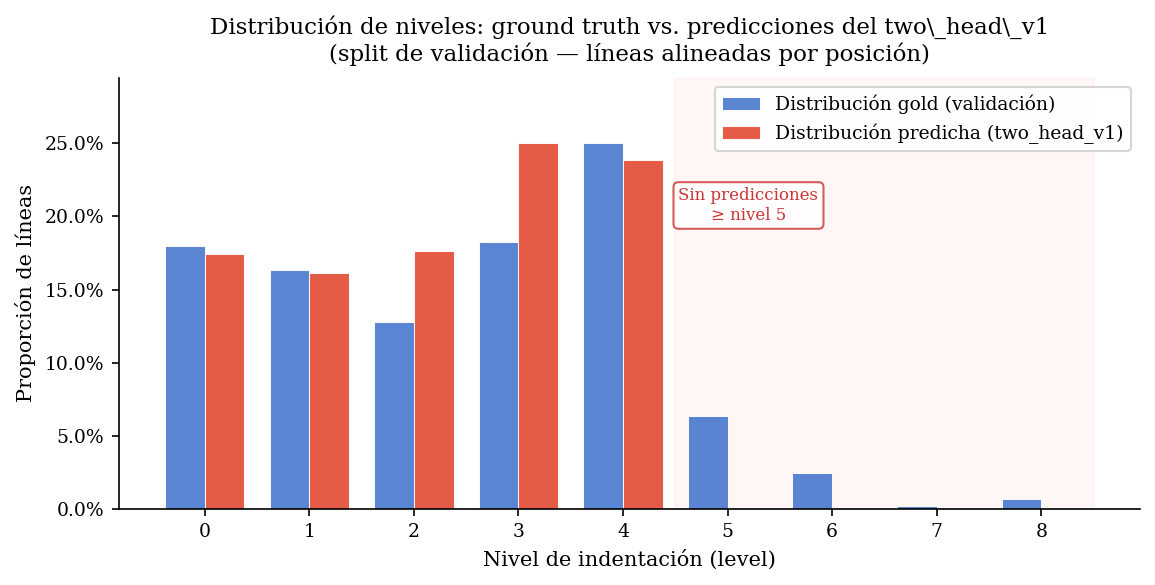
\includegraphics[width=0.82\textwidth]{figures/chapter6/fig6_5_level_distribution.png}
\caption{Distribución comparada de niveles: ground truth de validación (azul) y predicciones
         del \texttt{THM v1} (rojo). El modelo emite cero predicciones para los
         niveles 5 a 8; la zona sombreada marca la región de colapso.}
\label{fig:ch6_level_dist}
\end{figure}

Se puede vislumbrar un patrón claro: el cabezal de nivel del \texttt{THM v1} no emite ninguna predicción con valor mayor o igual a 5. De las 1800 líneas de validación, 174 tienen nivel
gold igual o superior a 5. Ninguna de ellas recibe una predicción correcta. El recall exacto para niveles 5--8 es del 0\,\%; el recall con tolerancia de un nivel (off-by-one) es del
28\,\%, lo que indica que el modelo se acerca a esos niveles desde abajo pero nunca cruza el umbral de decisión.

La causa estructural parecía ser el desbalanceo extremo de clases, un problema especialmente delicado cuando los valores raros no son categorías aisladas sino regiones poco frecuentes
de una variable ordenada o continua \citep{yang2021imbalancedRegression, steininger2021density}. El nivel 5 representa el 2,9\,\% de las líneas de entrenamiento. El nivel 6 el 2,6\,\%. El nivel 7 el 0,5\,\%. El nivel 8
el 0,1\,\%, lo que equivale a 8 líneas de entrenamiento sobre un total de 8336. Con una función de pérdida de entropía cruzada estándar y sin corrección de clase, el gradiente que
proviene de las instancias de nivel 8 es aproximadamente 115 veces más débil que el de las instancias de nivel 0. En la práctica, el cabezal aprende que es seguro ignorar los niveles
profundos: el coste de equivocarse en ellos es mínimo comparado con el coste de equivocarse en los niveles frecuentes.

Las muestras con parseo YAML fallido presentan una tasa de presencia de contenedores (\texttt{containers}) del 97,2\,\%,
frente al 79,4\,\% en las muestras parseables. Los manifests de tipo Deployment o StatefulSet son precisamente los que generan estructuras de nivel 5 o superior a través del
anidamiento \texttt{spec\textrightarrow{}template\textrightarrow{}spec\textrightarrow{}containers\textrightarrow{}volumeMounts}.


%----------------------------------------------------------------------
\section{Los modelos clasificadores ordinales}
\label{sec:ch6_ordinal}
%----------------------------------------------------------------------

El colapso hacia niveles superficiales está relacionado directamente con el tratamiento de la predicción de nivel como una clasificación categórica estándar. La entropía cruzada
multiclase no tiene noción del orden entre etiquetas: equivocarse entre nivel 3 y nivel 4 tiene el mismo coste que equivocarse entre nivel 3 y nivel 8. Pero en este contexto,
el orden importa.

La segunda familia de experimentos, denominada THO o variante ordinal versión 2, reformula la predicción de nivel como un problema de regresión ordinal. En lugar
de producir directamente una distribución sobre nueve clases, el cabezal proyecta el estado oculto a un escalar continuo $z$ mediante un MLP, y ese escalar se compara con una
secuencia de umbrales aprendibles $\tau_0 < \tau_1 < \ldots < \tau_7$ \citep{vargas2020cumulative}. El nivel predicho es el número de umbrales que $z$ supera:

\[
\hat{\ell} = \sum_{k=0}^{7} \mathbf{1}[z > \tau_k].
\]

La pérdida se define como la suma de entropías cruzadas binarias para cada uno de los ocho problemas de umbral: ``¿es el nivel mayor que $k$?''. Esta formulación obliga al modelo a
aprender una representación continua que respeta el orden entre clases, y permite que los umbrales sean aprendidos conjuntamente con el resto de la red. El objetivo es conseguir acceder
a los niveles profundos sin que el modelo tenga que aprender a predecirlos directamente como clases raras, sino a través de una representación latente que pueda cruzar umbrales de
forma más fluida.

Se probaron cuatro variantes dentro de esta familia, progresivamente modificadas en función de los diagnósticos obtenidos en cada run. La Tabla~\ref{tab:ch6_ordinal_variants} resume
los resultados de las cuatro variantes en el split de validación.

\begin{table}[htbp]
\centering
\caption{Comparativa de las cuatro variantes ordinales en el split de validación (70 muestras).
         La columna ``Recall exacto 5--8'' recoge el recall del cabezal sobre niveles profundos.
         La columna ``Off-by-1 profundo'' es el recall con tolerancia de $\pm$1 para niveles 5--8.}
\label{tab:ch6_ordinal_variants}
\begin{tabular}{lcccccc}
\toprule
\textbf{Variante}    & \textbf{YAML}   & \textbf{Nivel}  & \textbf{MAE}   & \textbf{F1}     & \textbf{Exacto} & \textbf{Off-1} \\
                     & \textbf{parse}  & \textbf{exacto} & \textbf{nivel} & \textbf{línea}  & \textbf{5--8}   & \textbf{5--8} \\
\midrule
initial              & 25{,}71\,\%     & 5{,}54\,\%      & 0{,}770        & 18{,}99\,\%     & 0{,}00\,\%      & 21{,}90\,\% \\
lr25 (thresh.\ ×25)  & 28{,}57\,\%     & 6{,}93\,\%      & 0{,}806        & 22{,}69\,\%     & 0{,}00\,\%      & 25{,}36\,\% \\
mlp3 (MLP 3 cap.)    & 14{,}29\,\%     & 4{,}09\,\%      & 0{,}918        & 11{,}53\,\%     & 0{,}00\,\%      &  0{,}00\,\% \\
centered (gap=0,5)   &  2{,}86\,\%     & 1{,}07\,\%      & 0{,}456        &  1{,}45\,\%     & 21{,}74\,\%     & 56{,}52\,\% \\
\bottomrule
\end{tabular}
\end{table}

\begin{figure}[htbp]
\centering
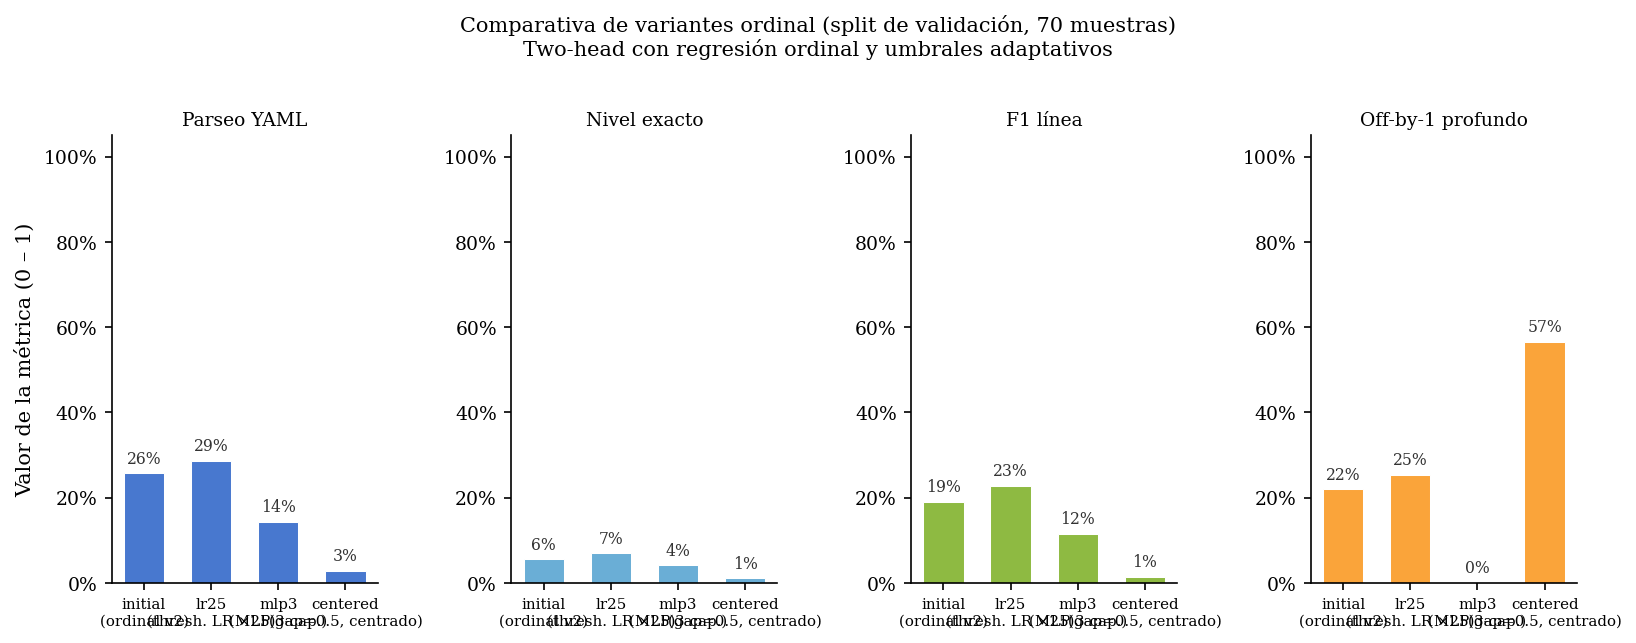
\includegraphics[width=\textwidth]{figures/chapter6/fig6_6_ordinal_variants.png}
\caption{Comparativa visual de las cuatro variantes ordinal en cuatro métricas:
         parseo YAML, coincidencia exacta de nivel, F1 de contenido textual y
         recall off-by-one en niveles profundos (5--8).}
\label{fig:ch6_ordinal_bars}
\end{figure}


%----------------------------------------------------------------------
\subsection{Variante inicial y tasa de aprendizaje de umbrales (lr25)}
\label{sec:ch6_ordinal_initial}
%----------------------------------------------------------------------

La variante inicial establece los umbrales con espaciado uniforme de 1,0 unidad ($\tau_0$ = 0,5, $\tau_1$ = 1,5, \ldots, $\tau_7$ = 7,5) y usa la misma tasa de aprendizaje
para todos los parámetros. Los resultados son peores que el THM v1 en parseo YAML (25,71\,\% frente a 48,57\,\%) pero no mejores en recall de niveles profundos:
seguimos sin conseguir que el modelo prediga ningún nivel mayor o igual a 5.

El diagnóstico de los umbrales revela que durante el entrenamiento completo (159 pasos), los umbrales apenas se desplazan. La variación total de $\tau_0$ a
$\tau_7$ es del orden de $10^{-3}$, mientras que el escalar latente $z$ oscila en un rango de $-$3 a +9. El modelo aprende ajustando $z$ y no los umbrales. La interpretación es que
el gradiente de la pérdida de umbral, pequeño en relación con el gradiente de la pérdida de contenido, es insuficiente para mover parámetros de umbral cuya inicialización ya permite
una clasificación aproximada de los casos frecuentes.

La variante lr25 multiplica la tasa de aprendizaje de los parámetros de umbral por un factor de 25 para intentar acelerar su ajuste. El resultado mejora marginalmente en parseo
(28,57\,\%) y en off-by-one profundo (25,36\,\%), pero los umbrales siguen sin desplazarse de forma significativa. El cambio en la tasa de aprendizaje produce un efecto observable,
pero no suficiente para romper el patrón de colapso.


%----------------------------------------------------------------------
\subsection{MLP de tres capas (mlp3)}
\label{sec:ch6_ordinal_mlp3}
%----------------------------------------------------------------------

La variante mlp3 aumenta la capacidad del cabezal de nivel a un MLP de tres capas con dimensiones (512, 256), lo que da al sistema más expresividad para proyectar el estado oculto
al escalar latente $z$. También aumenta el factor multiplicador de la tasa de aprendizaje de umbrales a 50. Los resultados no mejoran los anteriores experimentos: 14,29\,\% de parseo YAML y
un off-by-one de nivel profundo del 0\,\%. Seguramente esto se deba a un aumento de la capacidad del modelo sin mejoras en la entrada del entrenamiento ni en el número de muestras.


%----------------------------------------------------------------------
\subsection{Umbrales centrados: el primer acceso a los niveles profundos}
\label{sec:ch6_centered}
%----------------------------------------------------------------------

La variante \textit{centered-gap05} parte de una hipótesis diferente: si los umbrales se inicializan cerca de cero con espaciado estrecho (gap = 0,5, centrados en el origen:
$\tau_0$ = $-$1,75, $\tau_1$ = $-$1,25, \ldots, $\tau_7$ = +1,75), el escalar $z$ no necesita alejarse tanto de la región central para cruzarlos. En las variantes anteriores,
el umbral $\tau_4$ estaba en 4,5, lo que obligaba a $z$ a desplazarse mucho para predecir niveles altos. Con la inicialización centrada, cualquier pequeño movimiento de $z$ en la
dirección positiva puede activar predicciones de nivel profundo.

\begin{figure}[htbp]
\centering
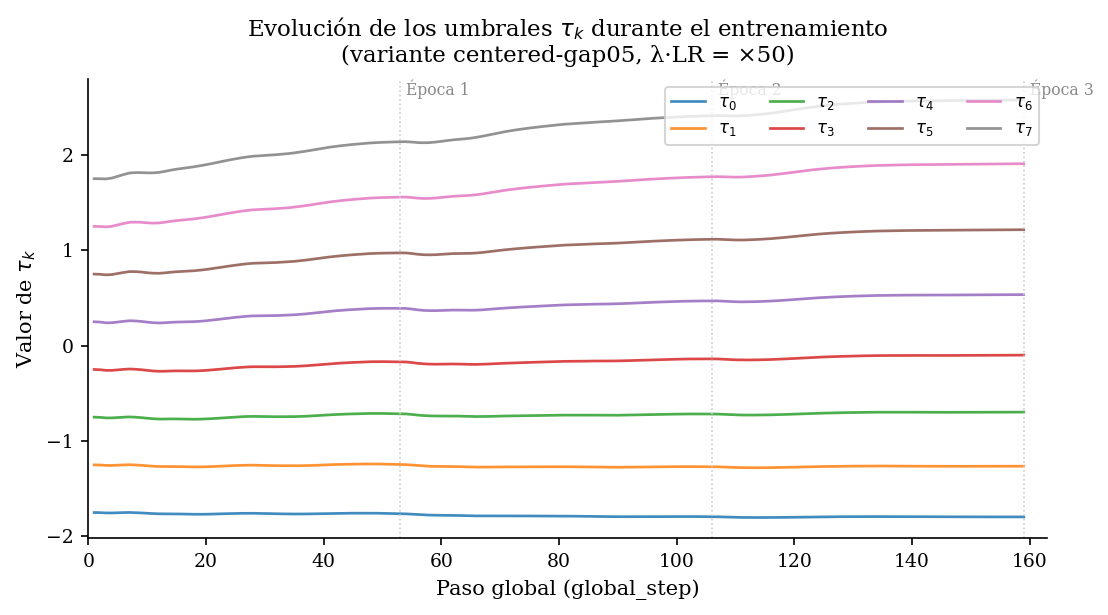
\includegraphics[width=0.82\textwidth]{figures/chapter6/fig6_7_threshold_drift.png}
\caption{Evolución de los ocho umbrales $\tau_k$ durante el entrenamiento de la variante
         \textit{centered-gap05} (159 pasos, 3 épocas). Los umbrales superiores a 4 se desplazan.}
\label{fig:ch6_threshold_drift}
\end{figure}

La Figura~\ref{fig:ch6_threshold_drift} muestra la evolución de los umbrales durante el entrenamiento. Parece que el aprendizaje sigue ocurriendo principalmente en $z$,
aunque los umbrales comienzan a moverse ligeramente.

Sin embargo, por primera vez en la familia de experimentos two-head, el modelo emite predicciones de nivel mayor o igual a 5. El recall exacto para niveles 5--8 es del 21,74\,\%, y
el off-by-one alcanza el 56,52\,\%, lo que indica que el sistema está activando predicciones en la zona profunda de la jerarquía de forma no trivial. Este resultado es cualitativamente
distinto al de todas las variantes anteriores: la señal existe, el cabezal puede aprender a cruzar los umbrales profundos si la inicialización lo facilita.

El coste, sin embargo, es severo. La tasa de parseo YAML cae al 2,86\,\% (2 muestras de 70). La F1 de línea se desploma al 1,45\,\%. El modelo genera predicciones de nivel profundo
pero pierde por completo la capacidad de generar estructuras correctas.
\begin{figure}[htbp]
\centering
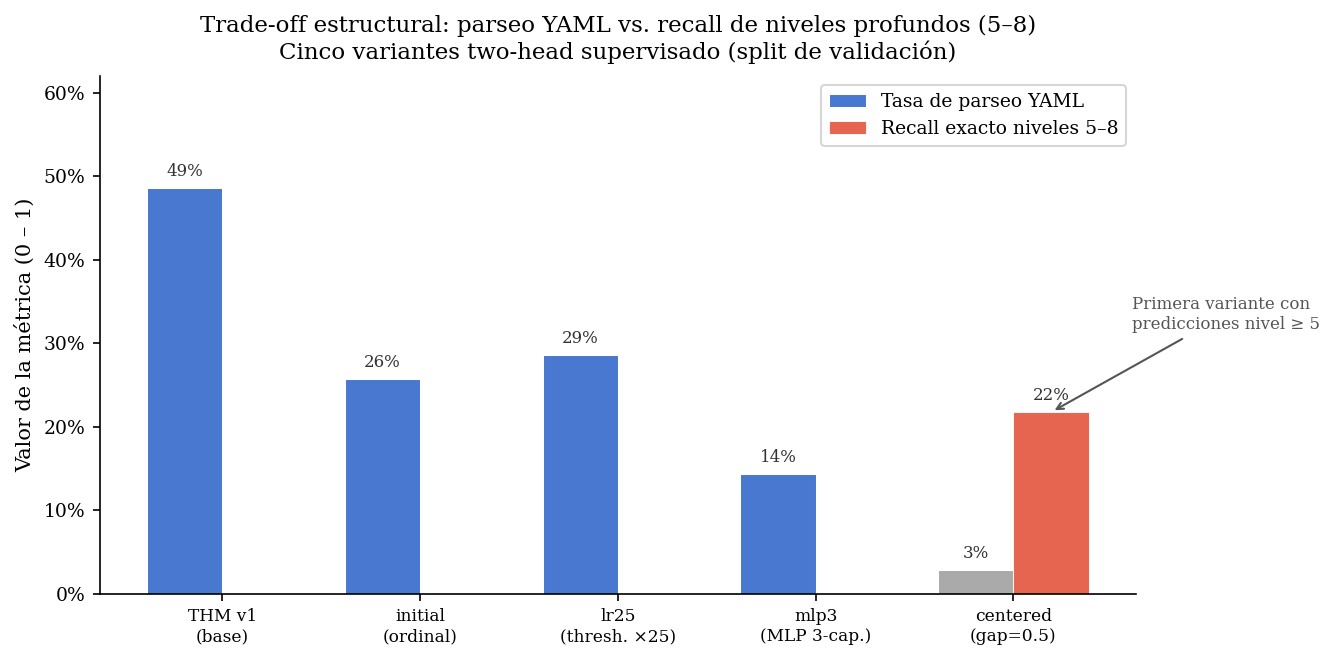
\includegraphics[width=0.85\textwidth]{figures/chapter6/fig6_8_structural_tradeoff.png}
\caption{Trade-off entre tasa de parseo YAML y recall exacto de niveles profundos (5--8)
         para las cinco variantes two-head probadas. Solo la variante \textit{centered} activa
         predicciones profundas, pero a costa de colapsar la generación de contenido.}
\label{fig:ch6_tradeoff}
\end{figure}

La Figura~\ref{fig:ch6_tradeoff} hace visible el trade-off de forma directa: ninguna variante consigue a la vez un parseo YAML razonable y un recall no nulo en los niveles profundos.
Las cinco variantes ocupan posiciones opuestas en ese espacio. El \texttt{two\_head\_v1} y las primeras variantes ordinales mantienen una tasa de parseo moderada pero recall profundo
nulo. La variante \textit{centered} activa el recall profundo pero destruye el parseo. No existe en el espacio explorado ninguna solución que haga las dos cosas a la vez.

\section{Análisis de errores del THO centrado}

A primera vista, el THO centrado podía leerse como una degradación clara: las métricas globales eran malas, el YAML generado era mayoritariamente inválido y la utilidad práctica del
modelo quedaba muy por debajo del THM v1. Sin embargo, precisamente porque esta variante consiguió activar niveles profundos por primera vez, debíamos de analizar que había ocurrido. El
análisis cualitativo de las salidas mostró que el problema no era solo la aparición de etiquetas raras, sino la posición en la que esas etiquetas aparecían dentro de la trayectoria
del manifiesto.
\label{sec:ch6_positional_drift}

El primer indicio apareció al comparar manualmente algunas predicciones de la variante \textit{centered-gap05} con sus referencias. En varios ejemplos, el contenido textual generado
era reconocible: aparecían recursos Kubernetes esperables, claves coherentes y secuencias de campos razonables. El problema estaba en la trayectoria de niveles que acompañaba a esas
líneas. De hecho, en los 24 ejemplos donde el número de bloques generado coincidía con el número de bloques de la referencia, el YAML reconstruido con los niveles predichos no
parseaba en ningún caso, mientras que al sustituir solo esos niveles por los niveles \textit{gold} parseaban 22 de los 24 ejemplos. Esta prueba no convierte la referencia en una
solución disponible durante inferencia, pero sí separa claramente dos causas: una parte importante del fallo no procedía del texto de las líneas, sino de la indentación estructural
que el cabezal asignaba a esas líneas.

Al inspeccionar esos fallos, el error no parecía distribuirse de forma uniforme a lo largo del manifiesto. El modelo no solo fallaba en los niveles profundos al final de la salida,
sino que tendía a retrasar la entrada en la jerarquía desde las primeras fases de generación. En otras palabras, mantenía demasiadas líneas en \texttt{level=0} cuando el YAML de
referencia ya había descendido a campos como \texttt{metadata}, \texttt{spec}, \texttt{selector} o \texttt{template}. Para comprobar esta hipótesis, cada
manifiesto se dividió en cuatro cuartiles relativos de longitud y se comparó la distribución de niveles predicha con la distribución real.

\begin{table}[htbp]
\centering
\small
\setlength{\tabcolsep}{4pt}
\caption{Distribución de niveles por cuartil en el análisis de errores del THO centrado.
         El patrón más relevante aparece en Q2: el YAML de referencia casi ya no está en
         \texttt{level=0}, pero el modelo conserva una proporción elevada de predicciones superficiales.}
\label{tab:ch6_quartile_level_drift}
\begin{tabular}{lccccc}
\toprule
\textbf{Tramo} & \textbf{Media gold} & \textbf{Media pred.} & \textbf{Gold nivel 0} & \textbf{Pred. nivel 0} & \textbf{MAE alineado} \\
\midrule
Q1 (0--25\,\%)   & 0,50 & 0,16 & 62,5\,\% & 89,5\,\% & 0,32 \\
Q2 (25--50\,\%)  & 2,32 & 1,39 &  1,8\,\% & 34,9\,\% & 1,10 \\
Q3 (50--75\,\%)  & 3,42 & 3,04 &  2,6\,\% &  3,5\,\% & 0,76 \\
Q4 (75--100\,\%) & 3,96 & 3,55 &  1,0\,\% &  1,7\,\% & 0,62 \\
\bottomrule
\end{tabular}
\end{table}

La Tabla~\ref{tab:ch6_quartile_level_drift} muestra la distribución de niveles por cuartil en el análisis de errores del THO centrado. En el primer cuartil es normal encontrar muchos niveles superficiales: todo manifiesto empieza con
campos como \texttt{apiVersion}, \texttt{kind} y \texttt{metadata}. Por eso el exceso de ceros en Q1 no es, por sí solo, la prueba más importante. El punto decisivo aparece en Q2.
Entre el 25\,\% y el 50\,\% de la secuencia, la referencia ya ha entrado de forma clara en niveles internos, pero el modelo todavía predice \texttt{level=0} en el 34,9\,\% de las
líneas. La lectura más precisa, por tanto, no es simplemente que el THO prefiera clases frecuentes, sino que su predicción de profundidad llega tarde: la estructura real desciende
antes de que el cabezal empiece a seguirla.

Esta observación llevó a formular el problema en términos temporales. La predicción de nivel no es una clasificación aislada de líneas independientes. Durante la generación
autoregresiva, cada paso produce un estado oculto de alta dimensión y, a partir de ese estado, el cabezal estima el nivel jerárquico correspondiente gracias a la representación $h$.
Si se denota por $h_t$ el
estado latente usado para predecir el nivel en la posición $t$, la salida puede entenderse como una serie temporal multivariante:

\[
(h_1, \ell_1), (h_2, \ell_2), \ldots, (h_T, \ell_T),
\qquad h_t \in \mathbb{R}^{3584}.
\]

Desde esta perspectiva, no hay razones para asumir que la distribución de los estados $h_t$ sea estacionaria a lo largo del YAML. Los estados del comienzo se calculan con menos
contexto generado, mientras que los estados posteriores incorporan una historia más larga de claves, listas, recursos y decisiones previas del propio modelo. Esto no significa necesariamente
que los estados iniciales sean peores o menos informativos. La hipótesis formulada va en otra dirección: el espacio latente sobre el que opera el cabezal de nivel cambia con la posición de
la línea, de modo que una misma etiqueta \texttt{level} puede ocupar regiones distintas al comienzo y al final del manifiesto. El cabezal ordinal, sin embargo, aprende una frontera
global que trata todos esos estados como si fueran muestras intercambiables de una única distribución.

Para comprobar si esta hipótesis tenía soporte, se reutilizaron los estados ocultos extraídos en el análisis latente previo y se calcularon distancias entre cuartiles
manteniendo fijo el nivel real. La estrategia más relevante fue \texttt{record\_prefix\_state}, porque es la misma política de lectura utilizada por el cabezal del THM. El resultado
fue significativo: para esa estrategia, la distancia media entre cuartiles dentro del mismo \texttt{level} fue prácticamente igual a la distancia media entre niveles distintos
dentro del mismo cuartil. En términos intuitivos, un estado de \texttt{level=2} al comienzo del YAML podía estar tan lejos de otro estado de \texttt{level=2} al final como de estados
pertenecientes a otros niveles. Esta es precisamente la situación en la que una frontera global puede quedar mal calibrada.

El análisis se reforzó con pruebas estadísticas sobre los mismos grupos. Primero, se aplicó MMD con kernel RBF para comparar Q1 frente a Q4 dentro de cada nivel con soporte
suficiente \citep{gretton2012kernel}. Todas las comparaciones evaluadas resultaron significativas tras corrección por comparaciones múltiples. Después, se aplicó PERMANOVA para comprobar si el cuartil
explicaba variación multivariante dentro de un mismo nivel \citep{anderson2001permanova}; de nuevo, el efecto apareció de forma sistemática. Finalmente, PERMDISP mostró que en muchos niveles la diferencia no
era solo un desplazamiento del centroide, sino también un cambio en la dispersión interna de los estados \citep{anderson2006permdisp}.

\subsection{Condicionamiento posicional del cabezal ordinal}
\label{sec:ch6_positional_encoder}

Con todo lo anterior aparece una solución bastante natural: si el espacio latente cambia con la posición de la línea, el cabezal de nivel no debería recibir únicamente el
estado oculto del modelo, sino también alguna señal explícita sobre el momento de la generación en el que se encuentra. Esta idea no pretende convertir la posición en una nueva
etiqueta ni multiplicar el problema en clases del tipo \texttt{level} por tramo posicional. La variable que se sigue prediciendo es el mismo nivel ordinal $\ell_t$. Lo que cambia es
la información disponible para estimarlo: además del estado latente $h_t$, el cabezal recibe una codificación causal de la posición absoluta de la línea generada.

Esto además es algo natural en el contexto de los Transformers, donde la codificación posicional es un componente estándar para que el modelo pueda distinguir entre posiciones
relativas y absolutas en la secuencia.

La primera variante se diseñó de forma simple. La posición utilizada es el índice de línea que se está generando, no la longitud final del manifiesto, por lo
que no introduce información no disponible en inferencia. Ese índice se transforma mediante una codificación sinusoidal de 16 dimensiones, siguiendo la intuición general de los
encodings posicionales de los Transformers y de las \textit{Fourier features} como mecanismo para representar coordenadas de baja dimensión \citep{vaswani2017attention, tancik2020fourierFeatures}, y se concatena justo antes de la proyección final del cabezal ordinal. De forma esquemática, la arquitectura
queda:

\[
\begin{aligned}
u_t &= f_h(h_t) \in \mathbb{R}^{64},\\
p_t &= f_p(t) \in \mathbb{R}^{16},\\
z_t &= w^\top [u_t; p_t] + b.
\end{aligned}
\]

Aquí $z_t$ es el score ordinal que después se compara con los umbrales aprendidos para obtener el nivel predicho. La rama $f_h$ proyecta el estado oculto mediante capas lineales,
normalización y activación no lineal, mientras que $f_p$ solo normaliza la codificación posicional sinusoidal. El objetivo de esta primera aproximación era comprobar si la señal
posicional efectivamente podía ayudar al modelo a activar niveles profundos a la vez que se mantenía un parseo YAML razonable.

\begin{table}[htbp]
\centering
\small
\setlength{\tabcolsep}{5pt}
\caption{Comparativa entre la base \textit{THO centered} y el primer experimento con codificación posicional por concatenación final (\textit{THOP v1}).
         La compresión de niveles 5--8 a 0--4 debe leerse en sentido inverso: valores más altos indican más colapso hacia niveles superficiales.}
\label{tab:ch6_positional_v1_final}
\begin{tabular}{lcc}
\toprule
\textbf{Métrica} & \textbf{THO centered} & \textbf{THOP v1} \\
\midrule
Predicciones de validación generadas & 70 / 70 & 70 / 70 \\
Ejemplos evaluados & 70 & 69 \\
Parseo de la salida estructurada & 100,00\,\% & 98,57\,\% \\
Parseo YAML & 2,86\,\% & 7,25\,\% \\
Exact match medio de nivel & 1,07\,\% & 2,23\,\% \\
MAE medio de nivel & 0,456 & 1,024 \\
Recall exacto en niveles 5--8 & 21,74\,\% & 13,79\,\% \\
Recall \textit{off-by-one} en niveles 5--8 & 56,52\,\% & 49,66\,\% \\
Compresión de niveles 5--8 a 0--4 & 60,14\,\% & 69,66\,\% \\
F1 medio de línea & 1,45\,\% & 4,55\,\% \\
F1 medio de requisitos del prompt & 1,43\,\% & 4,76\,\% \\
F1 semántico medio & 2,18\,\% & 6,38\,\% \\
KDV score medio & 2,38\,\% & 5,07\,\% \\
KDV gate pass & 0,00\,\% & 0,00\,\% \\
\bottomrule
\end{tabular}
\end{table}

\begin{figure}[htbp]
\centering
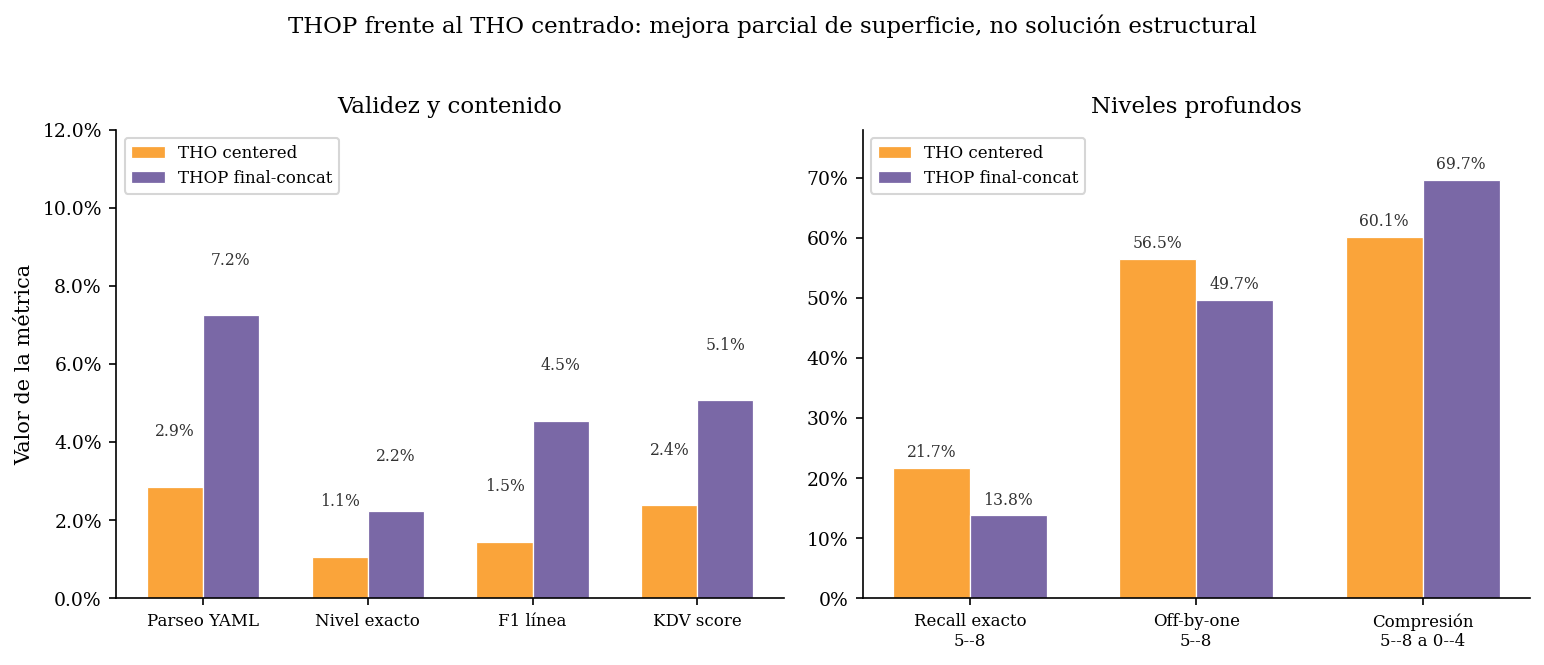
\includegraphics[width=\textwidth]{figures/chapter6/fig6_10_thop_metrics_comparison.png}
\caption{Comparación entre el THO centrado y el THOP con concatenación final. La compresión de niveles 5--8 a 0--4 debe leerse en sentido inverso:
         valores más altos indican más colapso de niveles profundos hacia niveles superficiales.}
\label{fig:ch6_thop_metrics_comparison}
\end{figure}

La Tabla~\ref{tab:ch6_positional_v1_final} y la Figura~\ref{fig:ch6_thop_metrics_comparison} muestran que la codificación posicional no resolvió el problema completamente. La tasa de
parseo YAML siguió siendo muy baja, aunque subió de 2,86\,\% a 7,25\,\% respecto al \textit{THO centered}, y también mejoraron las métricas de contenido y adecuación al prompt.
El diagnóstico por cuartiles confirmó además que el colapso inicial hacia \texttt{level=0} persistía: en el primer cuartil, el
modelo predijo \texttt{level=0} en el 94,7\,\% de las líneas, frente al 62,2\,\% de la referencia; en el segundo cuartil, donde la referencia solo tenía un 6,6\,\% de líneas en
\texttt{level=0}, el modelo todavía asignó ese nivel al 51,8\,\% de las líneas. Por tanto, el resultado no convierte a THOP v1 en una mejora global, pero sí indica que la posición
empieza a mover algunas métricas de reconstrucción, lo que justifica explorar formas de condicionamiento más expresivas.

\begin{figure}[htbp]
\centering
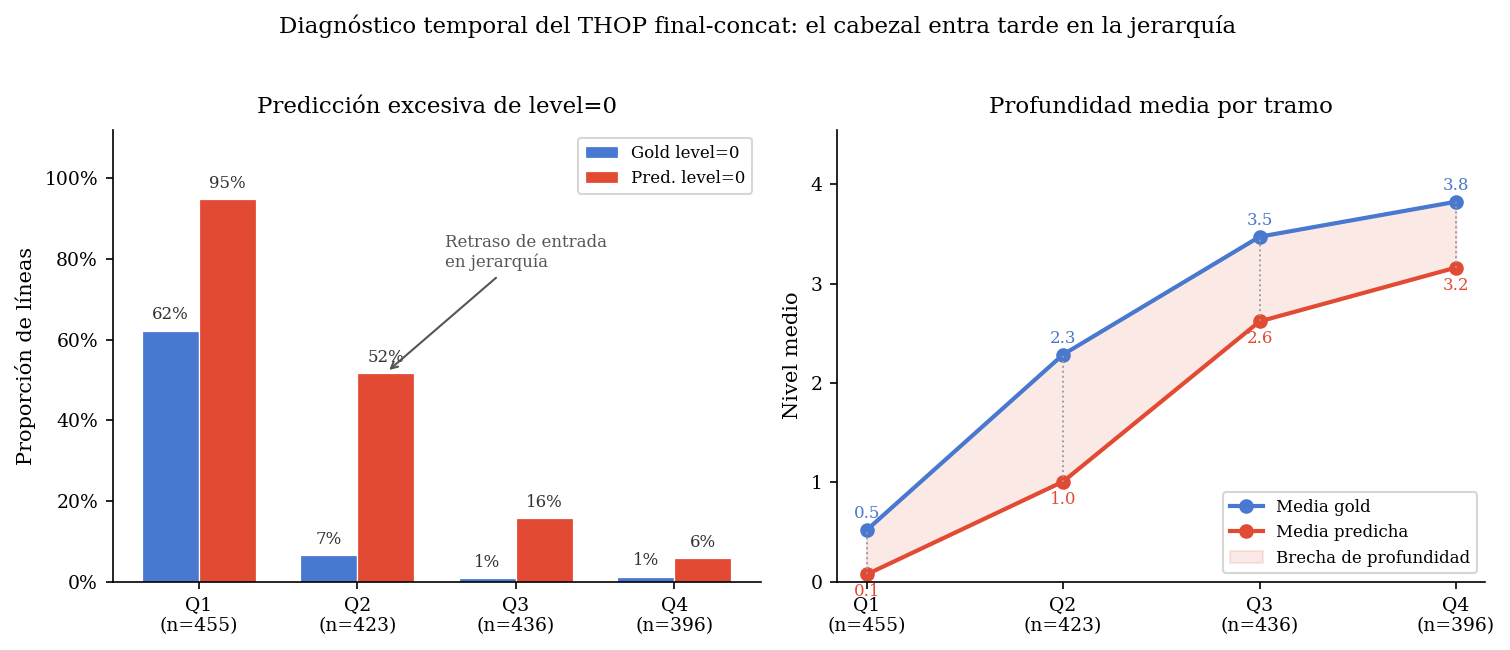
\includegraphics[width=\textwidth]{figures/chapter6/fig6_9_positional_v1_quartiles.png}
\caption{Diagnóstico por cuartiles del experimento THOP con concatenación final. La figura muestra, a la izquierda,
         el exceso de predicciones \texttt{level=0}; a la derecha, la brecha entre la profundidad media de la referencia
         y la profundidad media predicha.}
\label{fig:ch6_positional_v1_quartiles}
\end{figure}

También observé que el cabezal no fue simplemente ignorado. El análisis del proyector final mostró que la rama posicional tenía un peso no trivial: la norma
asociada a sus dimensiones representaba aproximadamente un 47\,\% de la norma de la rama latente. Además, la correlación entre la posición de línea y el score ordinal fue alta
($r=0{,}8460$). Con estos resultados vemos que la posición sí estaba afectando al score, pero lo hacía principalmente como una rampa temporal añadida
al valor ordinal. Dado que la interacción se produce en la última capa lineal, el modelo solo puede expresar una forma del tipo:

\[
z_t = w_h^\top u_t + w_p^\top p_t + b.
\]

En esta formulación, la posición corrige el score mediante un sesgo aditivo, pero no modifica la manera en que se interpreta el estado latente $h_t$. Y precisamente ahí parece estar
la limitación. La jerarquía YAML no es una función suave del índice de línea: una misma posición relativa puede contener una entrada en \texttt{metadata}, un descenso hacia
\texttt{spec.template}, un elemento de lista o una vuelta a un nivel menos profundo. Por eso, una señal posicional tardía puede aprender que, en promedio, las líneas posteriores
son más profundas, pero no necesariamente ayudar al cabezal a distinguir las transiciones estructurales locales.

\subsection{Segundo experimento posicional: modulación FiLM/gating}
\label{sec:ch6_positional_film}

El segundo experimento posicional parte de esa lectura. Si la concatenación final solo permite sumar un sesgo temporal al score $z_t$, la posición llega demasiado tarde: no puede
alterar la forma en que el cabezal interpreta las características internas del estado oculto. La alternativa es usar la posición como una condición que module las características
antes de la proyección ordinal final. Esta idea se apoya en mecanismos de transformación \textit{feature-wise}, especialmente FiLM, donde una señal condicionante genera parámetros
afines para reescalar y desplazar activaciones intermedias \citep{perez2018film}. La intuición de \textit{gating} es cercana: permitir que una señal auxiliar abra, cierre o atenúe
canales de representación en lugar de limitarse a sumarse al resultado final, una familia de mecanismos ya utilizada en modelos neuronales secuenciales \citep{dauphin2017language}.

En la variante THOP-FiLM, la posición de línea sigue siendo causal y absoluta, igual que en THOP. La diferencia está en el lugar de inyección. Primero, el estado oculto se proyecta a
un vector intermedio de 512 dimensiones. Después, la codificación posicional sinusoidal genera dos vectores, $\gamma_t$ y $\beta_t$, que modulan esas 512 características antes de
pasar al cuello de 64 dimensiones y al score ordinal. De forma esquemática:

\[
\begin{aligned}
r_t &= f_{\mathrm{pre}}(h_t) \in \mathbb{R}^{512},\\
(\gamma_t, \beta_t) &= g(p_t),\\
\tilde{r}_t &= r_t \odot \left(1 + \alpha \tanh(\gamma_t)\right) + \alpha \beta_t,\\
z_t &= f_{\mathrm{post}}(\tilde{r}_t).
\end{aligned}
\]

La inicialización también es importante. La última capa del generador FiLM se inicializa a cero, de modo que el modelo empieza cerca de una modulación identidad: al comienzo,
$\tilde{r}_t \approx r_t$. Esto evita que la nueva rama posicional destruya desde el primer paso la representación ya aprendida, pero deja espacio para que, durante el entrenamiento,
la posición aprenda a reponderar dimensiones concretas del estado latente.

El experimento final con esta variante se evaluó sobre las 70 muestras de validación. A diferencia del THOP por concatenación final, la salida estructurada fue parseable en todos los
casos, y la tasa de parseo YAML aumentó hasta el 28,57\,\%. Esta mejora es real respecto a las variantes ordinal-posicionales inmediatamente anteriores, pero queda lejos del 48,57\,\%
alcanzado por el THM v1. La Tabla~\ref{tab:ch6_film_positional_final} recoge las métricas principales del experimento.

\begin{table}[htbp]
\centering
\small
\setlength{\tabcolsep}{6pt}
\caption{Resultado final del experimento THOP-FiLM con modulación posicional sobre el cuello de 512 dimensiones.}
\label{tab:ch6_film_positional_final}
\begin{tabular}{lc}
\toprule
\textbf{Métrica} & \textbf{Valor} \\
\midrule
Predicciones de validación generadas & 70 / 70 \\
Ejemplos evaluados & 70 \\
Parseo de la salida estructurada & 100,00\,\% \\
Parseo YAML & 28,57\,\% \\
Exact match medio de nivel & 2,78\,\% \\
MAE medio de nivel & 0,843 \\
Recall exacto en niveles 5--8 & 12,14\,\% \\
Recall \textit{off-by-one} en niveles 5--8 & 41,43\,\% \\
Compresión de niveles 5--8 a 0--4 & 74,29\,\% \\
F1 medio de línea & 7,82\,\% \\
F1 medio de requisitos del prompt & 7,99\,\% \\
KDV score medio & 12,50\,\% \\
KDV gate pass & 0,00\,\% \\
\bottomrule
\end{tabular}
\end{table}

\begin{figure}[htbp]
\centering
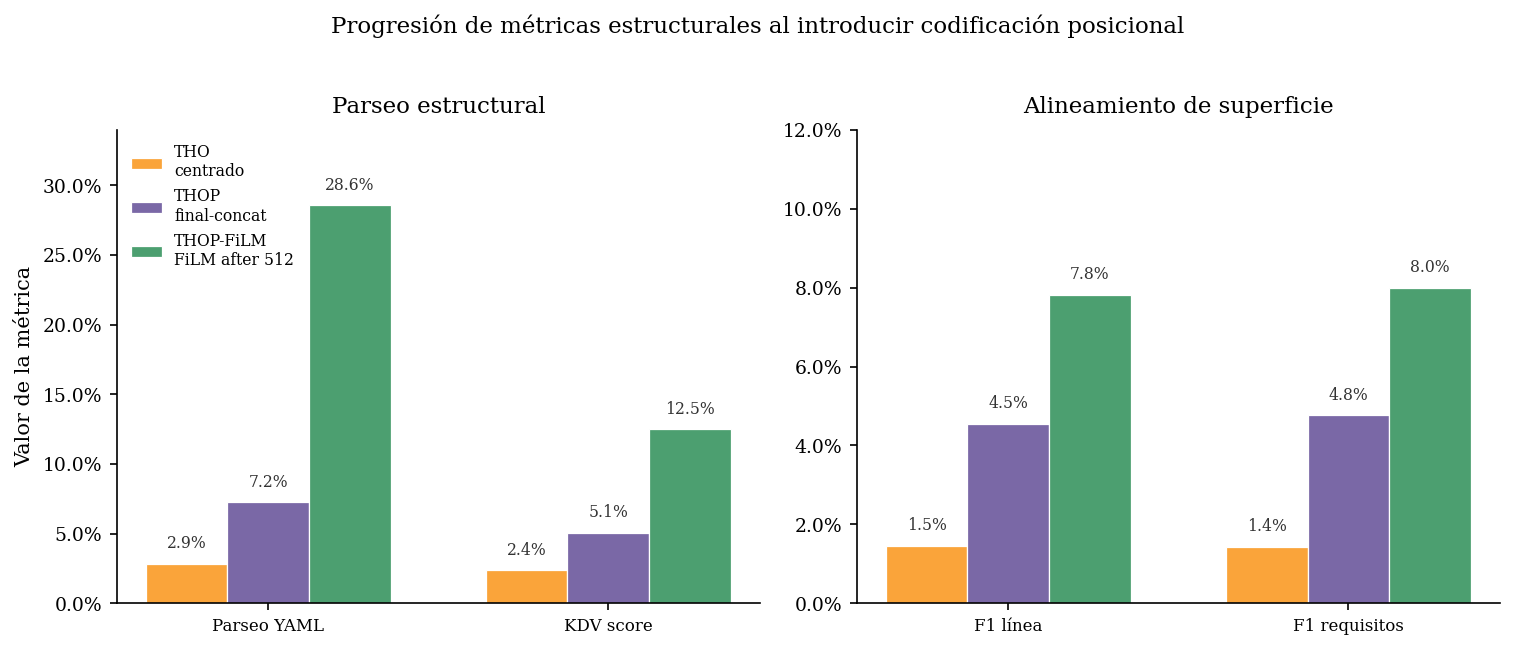
\includegraphics[width=\textwidth]{figures/chapter6/fig6_11_positional_parser_progression.png}
\caption{Progresión de métricas estructurales al introducir codificación posicional en el cabezal ordinal.
         El salto de THOP-FiLM es visible dentro de la rama ordinal-posicional, aunque sigue lejos del THM v1 en las métricas globales de validación.}
\label{fig:ch6_positional_parser_progression}
\end{figure}

La diferencia entre las dos variantes posicionales ayuda a sacar conclusiones. En la concatenación final, la posición actúa como un sesgo añadido al score ordinal. En THOP-FiLM,
en cambio, la posición modula las características intermedias antes de que el score se calcule. Esta segunda forma de interacción parece más adecuada que la concatenación tardía, porque
no fuerza a la posición a competir en la última capa con todo el estado latente, sino que le permite alterar la forma en que ese estado se interpreta. Aun así, el resultado no debe
leerse como una arquitectura ganadora: THOP-FiLM sigue degradando de forma severa el contenido, la exactitud de nivel y la parseabilidad global frente al THM v1. La conclusión más
prudente es que la posición sí contiene información útil para leer el estado latente, pero que incorporarla dentro de una formulación ordinal ya inestable no basta para recuperar un
generador robusto. Una línea natural para trabajo futuro sería volver al cabezal categórico del THM v1, que fue el mejor punto de la rama two-head en validación, y estudiar si un
condicionamiento tipo FiLM puede ayudarle a corregir su fallo específico en niveles profundos sin introducir el cuello de botella de un score ordinal único.

